\documentclass{article}
\usepackage{float}
\usepackage{hyperref}
\usepackage{graphicx} % Required for inserting images
\usepackage{multirow} % required for advanced tables
\usepackage[english]{babel}
\usepackage[T1]{fontenc}
\usepackage{textcomp}
%\usepackage{titlesec}
\usepackage{parskip}
\usepackage[margin=1in]{geometry}
\usepackage{color}
\usepackage{subfig}
%\usepackage{subcaption}

\graphicspath{{../figures/figures_report_3/}}

\title{ANALYSIS OF COVID-19 CHEST X-RAYS: \\Report 3: Final Report}
\author{Saniya Arfin, Yvonne Breitenbach, Alexandru Buzgan}
\date{June 2025}

\begin{document}

\maketitle

\tableofcontents

\newpage 

% ------------------------------------------------------------------------
% Chapter 1: Introduction
%------------------------------------------------------------------------
\section{Background and Project Motivation}
Medical imaging and particularly X-rays are one of the most important tools available to modern medicine in diagnosis and treatment of various diseases, due to their wide availability and cost-effectiveness.  The COVID-19 pandemic has highlighted the global need for such reliable, and scalable diagnostic means. In the case of COVID-19, the symptoms are similar to respiratory viral infections, and respiratory problems becomes the principal source of morbidity and mortality in advanced cases. Therefore, a quick and accurate detection of the virus infection could make the difference when fighting an epidemic of such proportions.\\
An important step in the diagnosis process is the interpretation of the image. This requires highly specialized professionals and it could be in many cases the bottleneck which prevents the quick diagnosis of large number of cases of respiratory diseases. Since this is basically a classification problem, Machine Learning and especially its subcategory Deep learning could prove to be a useful tool in this endeavor. Various Deep Learning models have demonstrated remarkable performance in image classification tasks, such as medical imaging diagnostics. Leveraging deep learning to analyze chest X-rays may provide an efficient and accurate method for detecting COVID-19 in patients, especially when traditional testing methods are not feasible.\\
This project explores the use of various models for classifying chest X-ray images into different categories, one of them being COVID-19. By training them on labeled X-ray datasets, the goal is to develop a reliable model that can assist healthcare professionals in identifying COVID-19 cases quickly and accurately.\\
As training data we use publicly available sets of X-ray images in a common image file format(PNG). The images were collected from different sources by a team of researchers from Qatar University, Doha, Qatar, and the University of Dhaka, Bangladesh along with their collaborators from Pakistan and Malaysia in collaboration with medical doctors. The sources of the images is mentioned in the reference section. The images are pre-labeled and contain:
\begin{itemize}
    \item X-ray images of healthy lungs (labeled 'Normal').
    \item COVID-19 positive cases
    \item  Viral Pneumonia positive cases.
    \item  Lung Opacity positive cases.
\end{itemize}
 
Our models will have to classify the images and especially detect the COVID-19 cases reliably. In this project we tested several Machine Learning and Deep Learning models in order to establish the best one for this task. We could not be exhaustive in our search, rather we selected the models with the best chances of obtaining a good result.\\
In the first step we tried to understand the dataset content and distribution, we identified and tried to address the data imbalance, biases and noises. We tried a few Machine Learning algorithms and then moved to Deep Learning algorithms, selecting the best one. We tried also pre-trained models specialized in image recognition. The metrics used for selection are the Confusion Matrix, which tells us how many images were correctly classified and the Classification Report which provides useful scores, most importantly the f1 score.\\
This report will detail our approach to this problem. We will start with a short description of the dataset. We will continue with a short list of the Machine Learning models we tested and a short description of hyper-parameter selection. Then we will continue with the Deep learning models we approached (including the pre-trained ones we used for transfer learning), we will detail the feature selection and finally draw conclusions and discuss about future work and possible improvements.  

%------------------------------------------------------------------------
% Chapter 2: Dataset Overview
%------------------------------------------------------------------------
\section{Dataset Overview - Description of the "Chest-X-Ray" Dataset}
The source of the dataset is \href{https://www.kaggle.com/tawsifurrahman/covid19-radiography-database} {Kaggle}. The size of the dataset is 1.15GB. It contains the following items:
\begin{itemize}
    \item a set of 3616  X-ray images of COVID positive cases.
    \item a set of 3616 mask images for the COVID images.
    \item a set of 6012  X-ray images of Lung Opacity positive cases.
    \item a set of 6012 mask images for the Lung Opacity images.
    \item a set of 10192  X-ray images of Normal (healthy) cases.
    \item a set of 10192 mask images for the Normal images.
    \item a set of 3616  X-ray images of Viral Pneumonia positive cases.
    \item a set of 3616 mask images for the Viral Pneumonia images.
    \item  4 Excel files containing metadata for each set of images
\end{itemize}

The metadata files contain the following information:
\begin{itemize}
    \item image size: all images sizes are mentioned here to be 256x256 pixels. However, the analysis showed that this is not accurate
    \item images format: all images are in the PNG format.
    \item image source: there are multiple sources for the images, as described below.
\end{itemize}

COVID-19 images:
\begin{itemize}
    \item 2473 images from padchest dataset[1]
    \item 183 images from a Germany medical school[2].
    \item 559 images from SIRM, Github, Kaggle and Tweeter[3,4,5,6]
    \item 400 images from another Github source[7]
\end{itemize}

Lung Opacity images:
\begin{itemize}
    \item all images are collected from Radiological Society of North America (RSNA) [8]
\end{itemize}

Normal images:
\begin{itemize}
    \item 8851 images are collected from Radiological Society of North America RSNA [8].
    \item 1341 images are from Kaggle [9].
\end{itemize}

Viral Pneumonia images:
\begin{itemize}
    \item all the images are collected from  the Chest X-Ray Images (pneumonia) database [9]
\end{itemize}

An example of each image is shown below:
\begin{figure}[H]
    \centering
    \begin{minipage}[t]{0.24\textwidth}
        \centering
        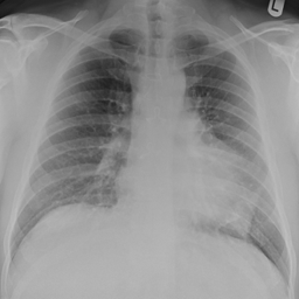
\includegraphics[width=\linewidth]{COVID-1023.png}
        \caption{COVID}
        \label{fig:COVID-1023.png}
    \end{minipage}
    \hfill
    \begin{minipage}[t]{0.24\textwidth}
        \centering
        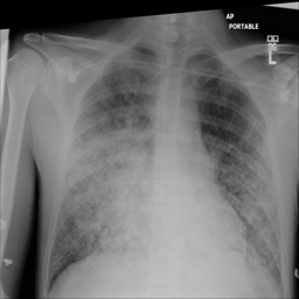
\includegraphics[width=\linewidth]{LungOpacity-1005.png}
        \caption{Lung Opacity}
        \label{fig:LungOpacity-1005.png}
    \end{minipage}
    \begin{minipage}[t]{0.24\textwidth}
        \centering
        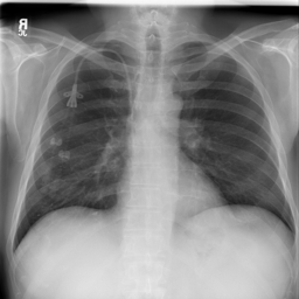
\includegraphics[width=\linewidth]{Normal-10023.png}
        \caption{Normal}
        \label{fig:Normal-10023.png}
    \end{minipage}
    \hfill
    \begin{minipage}[t]{0.24\textwidth}
        \centering
        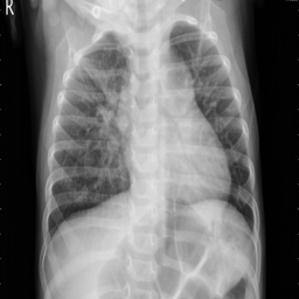
\includegraphics[width=\linewidth]{ViralPneumonia-1020.png}
        \caption{Viral Pneumonia}
        \label{fig:ViralPneumonia-1020.png}
    \end{minipage}
\end{figure}

The mask images isolate the lung area from the X-ray image. Each X-ray image has a corresponding mask which, if applied on the X-ray should leave only the lungs relevant area visible:
\begin{figure}[H]
    \centering
    \begin{minipage}[t]{0.48\textwidth}
        \centering
        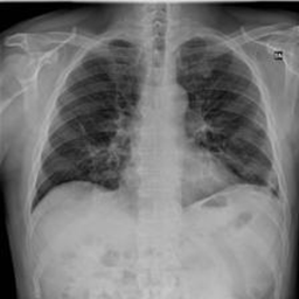
\includegraphics[width=\linewidth]{COVID-101.png}
        \caption{Image}
        \label{fig:COVID-101.png}
    \end{minipage}
    \hfill
    \begin{minipage}[t]{0.48\textwidth}
        \centering
        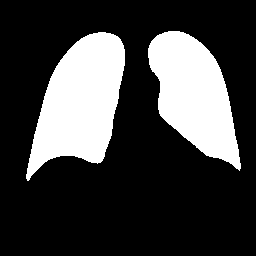
\includegraphics[width=\linewidth]{COVIDmsk-101.png}
        \caption{Mask}
        \label{fig:COVIDmsk-101.png}
    \end{minipage}  
\end{figure}

A first analysis of the images themselves shows that some information in the metadata files is wrong. The size of the images vary, as shown in the table below:
\begin{table}[h]
    \centering
    \begin{tabular}{|c|c|c|}
        \hline
        \textbf{Image size} & \textbf{Number of X-ray images} & \textbf{Number of lung masks} \\ \hline
        299 x 299 x 3 & 140 &  \\ \hline
        299 x 299 & 21025 &  \\ \hline \hline
        256 x 256 x 3 &  & 21165 \\ \hline
    \end{tabular}
    \caption{Size of X-ray images and lung masks}
    \label{tab:iamges_sizes}
\end{table}
Another problem is the format of the images: some are in RGB not grayscale. We had to take this into account during the data preparation phase.\\
The solution for the different sizes of the maska and images was a simple resizing of the masks to 299 x 299 pixel by using the resize-function of the OpenCV Python library. As interpolation method we used “cv2.INTER CUBIC”. This can be seen in detail in the overlay of some resized masks and X-ray images in figure \ref{fig:overlay_masks_images}.

\begin{figure}[h!]
    \centering
    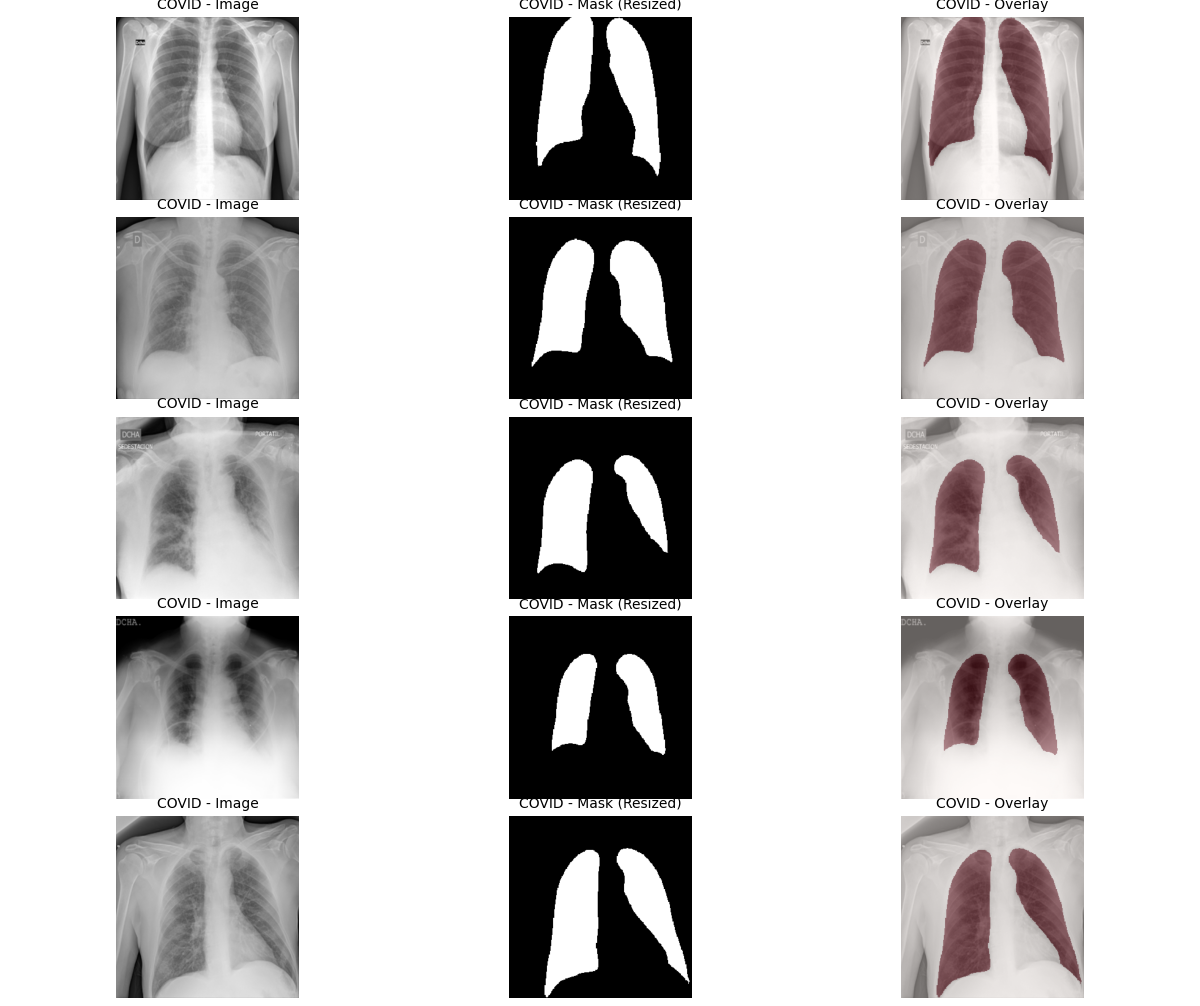
\includegraphics[width=1\linewidth]{overlay_masks_images.png}
    \caption{Overlay of resized masks and X-ray images.}
    \label{fig:overlay_masks_images}
\end{figure}   

The next step in our analysis were the exploratory data visualizations. We created class-wise and source-wise smoothed Kernel Density Estimate (KDE) plots for mean pixel intensities and for standard deviations (std) of pixel intensities. The conclusion was that different classes show distinct mean intensity patterns. COVID images tend to be brighter on average, potentially due to artifacts or progression patterns, while Lung Opacity images are darker. Also the images have significantly different mean and standard deviation values of pixel intensities across the four classes. This variation reflects inherent differences in image acquisition conditions or dataset characteristics (for example, images taken with different machines or in different settings may have varying brightness and contrast levels), which could introduce bias into any Machine Learning model.\\
To minimize source-related bias and standardize image quality across the dataset, we applied the following preprocessing steps:
\begin{itemize}
    \item Grayscale Conversion (L-channel): All images were converted to grayscale using OpenCV (RGB conversion to L).
    \item Contrast Enhancement with Contrast Limited Adaptive Histogram Equalization (CLAHE): Applied CLAHE to help standardize the contrast across images.
    \item Lung Region Isolation: By applying the binary mask to the image after CLAHE processing, we ensured that only the lung regions are enhanced and normalized, while irrelevant areas like the background are not affected.
     \item Pixel Value Normalization: Ensures that all images lie within the same range, preventing models from learning biased patterns based on intensity differences.
\end{itemize}

Figures \ref{fig:KDE_pre_post_normalization_class} and \ref{fig:KDE_pre_post_normalization_URL} show the effect of the normalization. 

\begin{figure}[h!] % the [h!] helps force it "here"
    \centering
    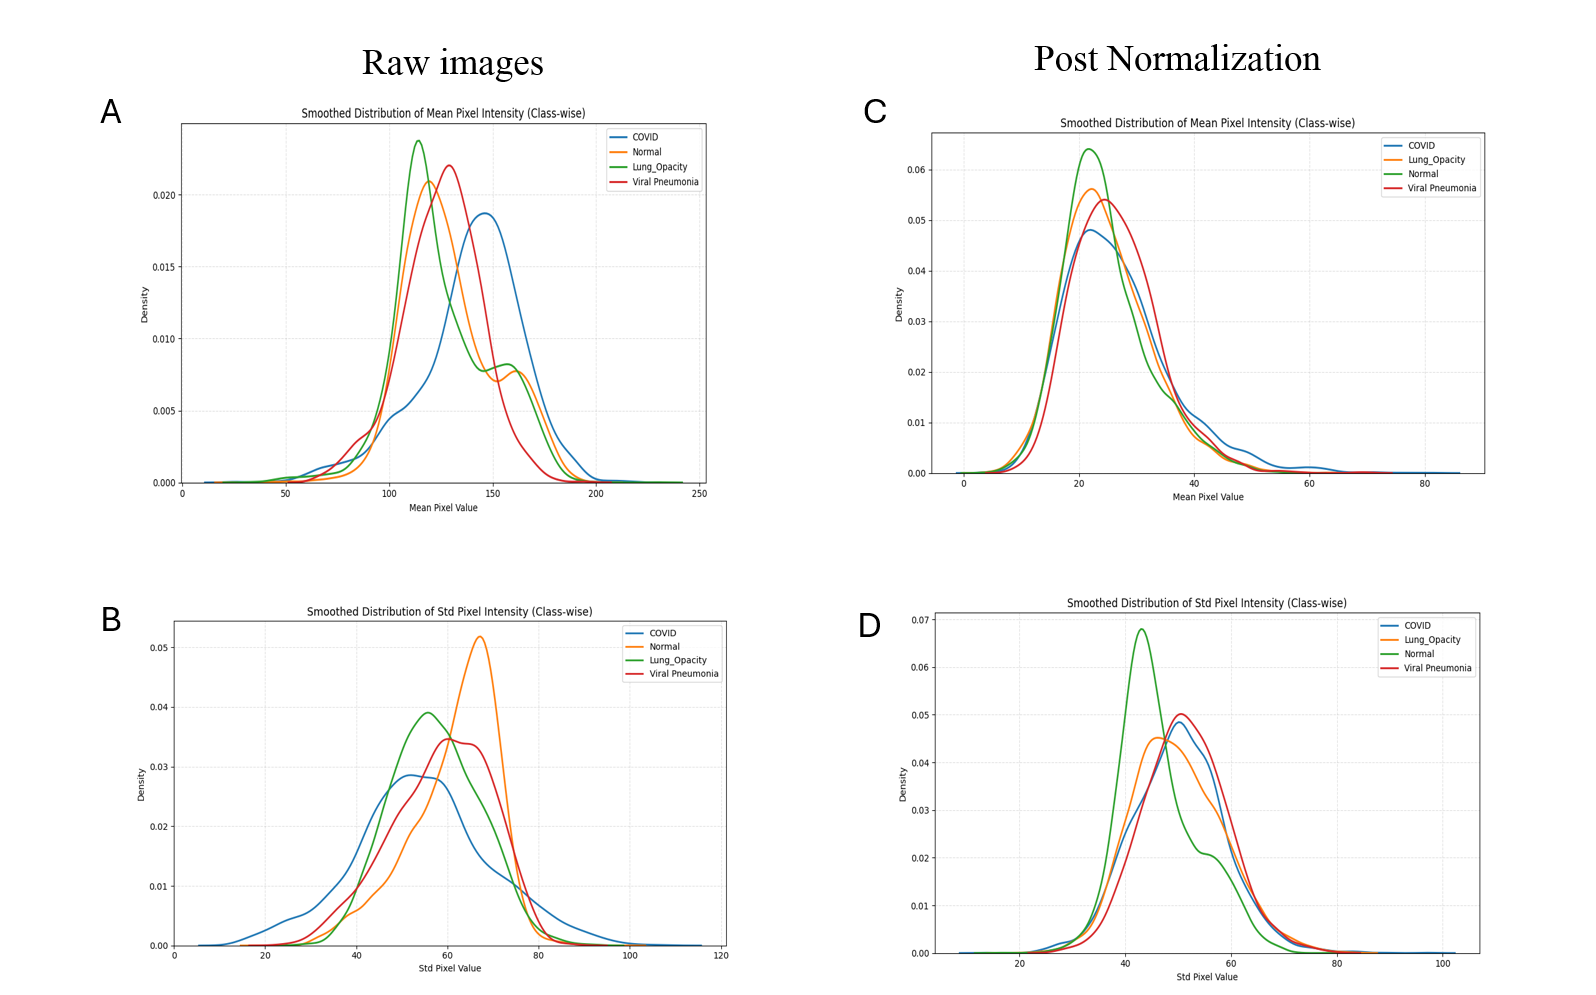
\includegraphics[width=1.0\linewidth]{Screenshot 2025-04-21 223200.png}
    \caption{Distribution of mean and std of pixel intensities of the X-ray images before and after normalization by classes}
    \label{fig:KDE_pre_post_normalization_class}
\end{figure}

\begin{figure}[h!] % the [h!] helps force it "here"
    \centering
    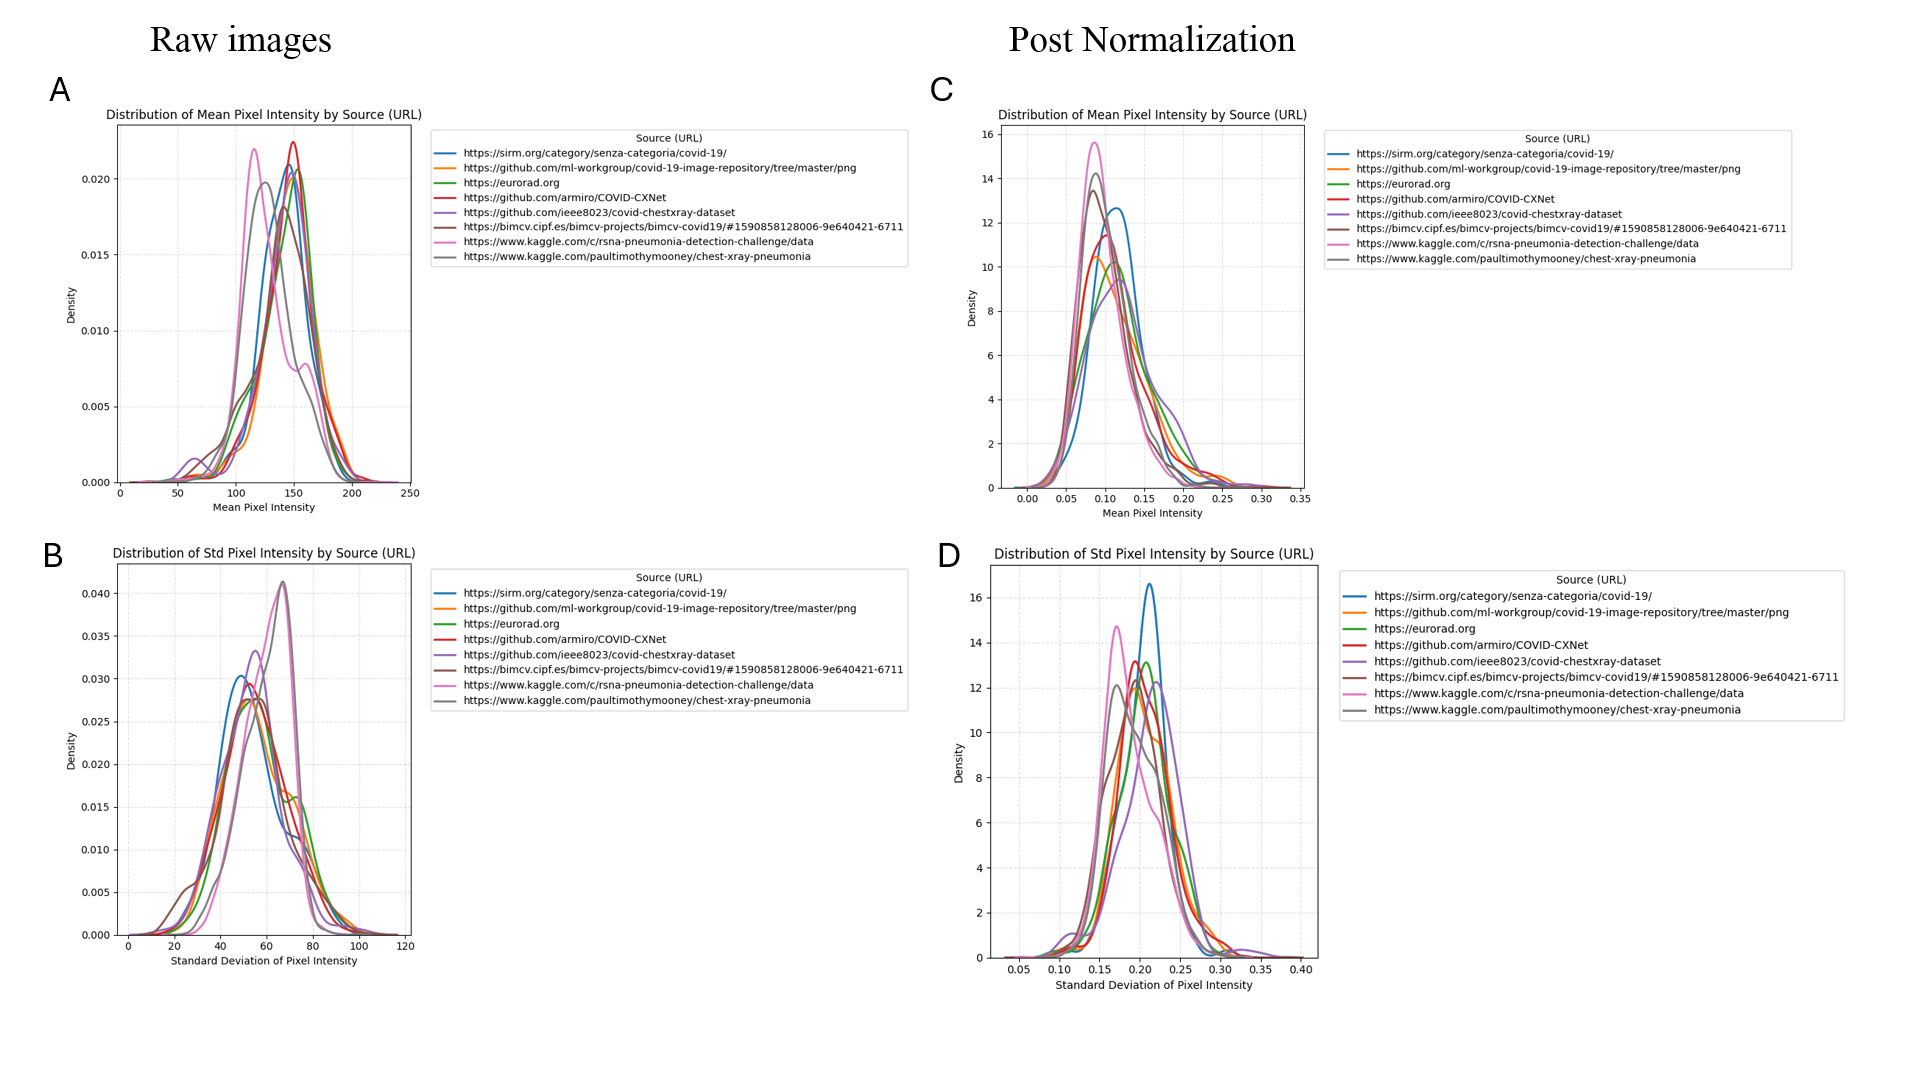
\includegraphics[width=1.0\linewidth]{Screenshot 2025-04-21 223207.png}
    \caption{Distribution of mean and std of pixel intensities of the X-ray images before and after normalization by sources}
    \label{fig:KDE_pre_post_normalization_URL}
\end{figure}

The preprocessed images are converted to numpy arrays and stored as .npz files for fast loading during training and evaluation.


%------------------------------------------------------------------------
% Chapter 3: Methodology - Modelling
%------------------------------------------------------------------------
\section{Modelling} \label{section:modelling}


%------------------------------------------------------------------------
% 3.1 : Overview of modeling
%------------------------------------------------------------------------
\subsection{Overview of the modeling}
This chapter summarizes the modeling carried out in this project. Not all modeling runs which have been performed are described. These can be found in our 2nd report: "Second\_report.Covid\_xray.pdf". Here we focus on presenting the essential modeling steps for each model used. In addition, the best results of each model are presented. 

In this project we used a two-step approach to solve this classification task. Initially, we applied machine learning techniques to extract meaningful insights. The models used were “Logistic Regression”, “Random Forest”, “Support Vector Machines” and “XGBoost”. As a transition to deep learning, we also tried out “MLP-Classifier”. For the tests with the machine learning models, we prepared the input data in different ways so that we had different data sets that we could try out. This data preparation had been done previously to training. 

As a second step, we tried to solve this classification task with deep learning models. On the one hand, we used a self-build lightweight Convolutional Networks (CNN). On the other hand, we applied transfer learning. Therefore, the following pretrained models from KERAS were used: EfficientNet, InceptionV3, DenseNet121 and VGG16. Finally, we combined two different deep learnin models to an ensemble model. We tried to apply these models with and without fine-tuning to our data. 

%------------------------------------------------------------------------
% 3.2 : Machine Learning Tequniqes
%------------------------------------------------------------------------

\subsection{Step 1: Machine Learning Models}
We started with traditional machine learning algorithms. We already had in mind that these models might not be the best choice to solve a classification task of chest X-ray images. However, it was worth a try to test them because they have a big advantage over deep learning models: They are computationally inexpensive and we can quickly iterate over different versions, features and preprocessing methods. The models we employed included:

\begin{itemize}
    \item Logistic Regression – A well-known method for classification problems.
    \item Random Forest – An ensemble method that builds multiple decision trees to improve accuracy and handle complex relationships in the data.
    \item Support Vector Machines (SVM) – A technique that finds the optimal boundary between different categories.
    \item XGBoost – A powerful algorithm that is known for its accuracy and speed and can handle large datasets.
    \item MLP Classifier – A simple neural network that captures non-linear relationships but remains limited compared to deeper architectures.
\end{itemize}

%------------------------------------------------------------------------
% 3.2.1 : Logistic regression
%------------------------------------------------------------------------

\subsubsection{Logistic Regression}
With the Logistic Regression model 6 different model runs were performed. On the one hand, the images themselves were used as input data. For performance reasons, however, they had to be significantly reduced in size (only 20x20 pixels). For another run, filtering methods were applied to these X-ray images. In another run, additional masks were added to the images to obscure the areas outside the lungs. This should help to focus the model on the important areas. 
For another model run not the images themselves had been used as input data. Before the modeling, the HOG-technique (Histogram of Oriented Gradients) had been applied to extract structural patterns from the grayscale X-ray images. HOG captures from X-rays
\begin{itemize}
     \item edges of lung boundaries, rib cage, and lesions
     \item orientation and distribution of densities i.e. darker/ lighter areas correspond to tissue and opacity differences
     \item shape and spread of abnormalities, like how diffuse or sharp an opacity is
\end{itemize}
Although HOG is handcrafted, not learned  and  so it may miss subtle texture or high-level patterns, it is a fast, interpretable, and memory-efficient way to extract features from chest X-rays. 
Aditionally we compressed the HOG features by a PCA (Principal Component Analysis) and finally we tried to optimize the model's hyperparameters. 

With a Logistic Regression model the best overall accuracy we achieved was 73.7\% using the HOG-extracted features as input data. This model run also made the best predictions for the COVID class (using a Logistic Regression model). The scores were:  precision: 52\%, recall: 56\% and f1-score: 54\%. This result leaves room for improvement. Logistic regression might not be the best choice for such a high-dimensional feature set.\\


%------------------------------------------------------------------------
% 3.2.2 : Random Forest
%------------------------------------------------------------------------

\subsubsection{Random Forest}
From the various experiments with the Logistic Regression model, we have already seen that the use of the HOG features as input data were the most promising model rus. Therefore, the tests with the Random Forest model started directly with the HOG-features as input data. 

With the random forst model 2 different model runs were performed: One with the model's default hyperparameters. And the second run used optimized hyperparameters found by using the GridSearch-technique. This optimization of the hyperparamters brought a slight improvement. We thus achieved an overall accuracy of 76\% with the Random Forest model. Also, the prediction of the COVID class could be slightly improved (precision: 62\%, recall: 61\% and f1-score: 62\%) copared to our best Logistic Regression model.

%------------------------------------------------------------------------
% 3.2.3 : Support Vector Machines (SVM)
%------------------------------------------------------------------------

\subsubsection{Support Vector Machines (SVM)}
As the model runs with the Random Forest model slightly imroved the previous predictions made with the Logistic Regression model, we wanted to test if the use of another model could further improve the predictions. We performed 7 more or less sucessful model runs with SVM model. 
With the SVM model, we first wanted to check again the qualitiy of the predictions when we use the images themselves. Therefore, we did not immediately start with the extracted features. The first test had already shown that we needed to drastically reduce the size and number of images when using a SVM model. A test using all images (augmented and non-augmented, approx. 35000 images) reduced to 128 x 128 pixels was aborted after 6 hours. As it took that much time even without using a hyperparameter optimization technique like GridSearchCV, we needed to change the dataset (number or/ and size of images) for further tests. 

Further runs in which we changed the size and number of images, and tested different hyperparamater optimization techniques showed that, for performance reasons, we could only use a very small number of images (1000 per class) with a resolution of 128 x 128 pixels. This resulted in the highest overall accuracy (57\%) we could achieve with an SVM model using the images themselves. However, the results for the COVID class were not satisfactory (precision: 45\%, recall: 43\% and f1-score: 44\%). The time needed to fit the model was about 1 hour, which is a lot for such poor prediction results. Maybe the model would perform better if more images or more pixels per image would be used. But due to the long training times we considered a training with more images not as an option.

Therefore, we decided to use already extracted features as input data of the SVM models, because this had already revealed better results when using other machine learning models like Random Forest and Logistic Regression. In conclusion of various tests, using Hog-features with PCA dimensionality reduction gave us SVM model's the best accuracy of 77\% and for the COVID-class (precision: 59\%, recall: 63\% and f1-score: 61\%). These results are comparable to those of the best Random Forest model.

%------------------------------------------------------------------------
% 3.2.4 : XGBoost - Extreme Gradient Boosting
%------------------------------------------------------------------------

\subsubsection{XGBoost - Extreme Gradient Boosting}
As XGBoost - models (Extreme Gradient Boosting) are known for handling large datasets efficiently we gave this a try. We performed 5 different test runs with a XGBoost - model. 

As a first step, we tested the performance of an XGBoost model against the previously utilized SVM model using the same input data (4000 images with 128 × 128 pixels). XGBoost significantly outperformed SVM in terms of efficiency, completing the task in just 5 minutes compared to SVM’s 1-hour runtime. Furthermore, the accuracy of the XGBoost prediction was much better. 
Building upon these promising results, we extended our dataset for further XGBoost runs, increasing the number of images by using all images (including both augmented and non-augmented iamges, approx. 35000) while maintaining the same image resolution.

For furhter runs we explored multiple variations of input data. These included combinations of applying and omitting masks, using and not-using filters. The highest overall accuracy of 86\% was achieved with an XGBoost model trained on the full dataset, without masks or filters. Notably, the classification performance for the COVID-class reached impressive 89\% for precision, recall and f1-score, marking our best results so far with a machine learning model.

Although models such as Random Forest, Logistic Regression, and SVM demonstrated improved predictive accuracy when utilizing pre-extracted features as input data, this was not the case for XGBoost model. Despite expectations, HOG-features did not yield superior results compared to using the images themselves.

%------------------------------------------------------------------------
% 3.2.5 : MLP-Classifier
%------------------------------------------------------------------------

\subsubsection {MLP-Classifier} 
As a transition to deep learning, we also tried out the Multi-layer Perceptron classifier model (MLP-Classifier), which is a simple neural network. 

Overall we performed 7 runs with an MLP-Classifier which involved modifications of the model's architecture/ layers, activation functions, class weights and learning rate. Although the overall accuracy of these runs was not too bad (77-78\%), the COVID class could not be predicted well. Therefore, we tried to work on the input data and used techniques like SMOTE (Synthetic Minority Over-sampling Technique) and focal loss to help to balance the class distribution. But the COVID-class was still underperforming. 

HOG-extracted featues were used for the previous tests with the MLP classifier. To further improve the predictions, an attempt was made to use features that were extracted with a ResNet model. ResNet is a deep convolutional neural network pretrained on ImageNet. It learns hierarchical, high-level features (like textures, shapes, patterns) that are often more effective than handcrafted ones. With this we achieved the best accuracy (82.8\%) with a MLP classifier model. The Covid class was still difficult to predict, the recall: was only 69\%, but the predictions (recall) for the other classes were better: Lung Opacity: 78\%, Normal: 89\%, Viral Pneumonia: 94\%.
During training, we observed signs of overfitting. To counteract this L2 regularization (Ridge Regularization) was introduced and the number of neurons was reduced. Despite these adjustments, while overfitting was reduced, the accuracy did not improve.

%------------------------------------------------------------------------
% 3.3 : Deep Learning
%------------------------------------------------------------------------

\subsection{Step 2: Deep Learning Models}

We have already performed many runs with several traditional machine learning models based on different preprocessed input data. A XGBoost model on 128 x 128 images without masks, no filter (Clahe, Gaussian Blur) gave us the best overall accuracy of 86\% so far. This model's classification performance for the COVID-class reached impressive 89\% for precision, recall and f1-score. Now it is time to move on to try if Convolutional Neural Networks (CNN) can improve the accuracy of the predictions on our chest X-ray dataset. 

Deep learning offers significant advantages over traditional machine learning for classifying chest X-ray images. These models excel in handling high-dimensional data and they can automatically identify relevant features. Deep learning models, particularly convolutional neural networks (CNNs), learn features directly from raw image data, so that no preprocessing like feature extraction and applying relevant filters has to be done by hand. This ability allows them to capture subtle patterns and complex structures that may be missed by manually designed features.

%------------------------------------------------------------------------
% 3.3.1 : Self-build CNN model
%------------------------------------------------------------------------

\subsubsection{Self-built CNN model} 
We started into modeling with deep learning by building our own small CNN. As a main part our CNN contains 3 convolutional blocks, each containing the following layers: 
\begin{itemize}
    \item Convolutional Layer
    \item Bacht normalization layer
    \item Activation layer
    \item MaxPooling2D layer
\end{itemize}
In simple words: With these convolutional blocks the model "learns" from the input X-ray images and step by step extracts the relevant features in order to solve the classification task. 
Overall, the model achieved an accuracy of 92\%. When broken down by class, the model performed particularly well on the COVID and Viral Pneumonia categories. For COVID cases, it attained a precision of 93\%, a recall of 98\%, and an F1-score of 95\%, indicating both high correctness and sensitivity in identifying positive cases. 

Even with this quite simple self-built CNN, we achieved better results than with all previous attempts using machine learning models. In the following tests we focused on using CNNs, which have been pretrained on other images, and partly re-trained them on the chest X-ray images from our own dataset.

%------------------------------------------------------------------------
% EfficientNet
%------------------------------------------------------------------------

\subsubsection{EfficientNet} 
The model runs with the EfficientNet model revealed, that not all deep learning models show better results than we achieved during our test with the machine learning models. 
The COVID class suffered from poor recall (0.07) and low precision (0.28), yielding a very weak F1-score of 0.11, which suggested significant difficulty in correctly detecting COVID cases. Overall, the model attained an accuracy of only 58\%. Given the low recall and F1-scores for these critical classes, we decided not to move forward with this model and instead explored other approaches to improve classification performance.

%------------------------------------------------------------------------
% InceptionV3
%------------------------------------------------------------------------

\subsubsection{InceptionV3} \label{section:InceptionV3}

As the first attempts using a pretrained InceptionV3 model showed very poor results, we performed several model runs with modifications of the used input data. Therefore, the data processing was adapted to be done dynamically before training, rather than offline, allowing easier modifications. As initial augmentation attempts of the training dataset led to poor Normal-class predictions, we concluded that for this model the imbalance has to be corrected by augmenting images across all classes (including the normal class) not just the minority ones. Using these input data led to more promising results, so that we used this dataset as input data for the model runs with the InceptionV3 model. 

At first, we tried to use the pretrained InceptionV3 model as it is, without retraining some layers on our chest X-ray dataset. We performed 8 major runs with the InceptionV3 model. During these tests we changed different parameters like the batach size, number of epochs, laerning rate, the optimizer and used callbacks to automatically reduce the learning rate during training. The results of all of these model runs were not satisfying. The accuracy of the predictions was not as high as of other models. Beyond that, looking at the evolution of accuracy and loss over the different epochs of training, there is a lot of oscillation. This indicates that the model does converge which does not give us confidence in this model. 

As a next step we tried to unfreeze several layers of the pretrained model in order to retrain and adapt them to our X-ray dataset. First we tried to unfreeze only the last 4 layers and then even tried to unfreeze a lot more layers (about 60 of 311 layers) - as suggested in several online sources. This run achieved an overall accuracy of 91\% and even the COVID-class is well predicted (precision 92\%, recall 91\% and f1-score 91\%). 

As this looks quite promising, we repeated this test and tried to improve the predictions by apllying the corresponding attention masks to the X-ray images. This could help the deep learning model to focus only on the relevant areas of the images: the lungs. We tried 3 different datasets, by applying the masks only to the train dataset, to the train and validation dataset and finally to the train, validation and test dataset. The 3rd attempt, where the masks were applied to the train, validation and test dataset, showed the only useful results. However, the overall accuracy was less with only 84\% and also the predictions for the COVID class are worse than without masks. 


%------------------------------------------------------------------------
% DenseNet121
%------------------------------------------------------------------------

\subsubsection{DenseNet121} 
As we had already carried out very extensive tests with the InceptionV3 model, we saw no further room for improvement with this model. We therefore wanted to test another model: DneseNet121. Three different runs have been performed using a pretrained DenseNet121 model. During these runs we tried to improve the accuracy by: 
\begin{enumerate}
    \item changing the size of the input images (64x64 and 224x224 pixel)
    \item adding extra pre-processing layers before the pretrained DenseNet121 model 
    \item adding more dense layers after the pretrained DenseNet121 model.
\end{enumerate}

The third run showed the highest overall accuracy (85\%) we got with a DenseNet121 model. Unfortunately, the worst predicted class is COVID: precision 73\%, recall 78\% and f1-score 76\%. 
We achieved less good results with the DenseNet121 model than with other models. Nevertheless, the diagram of loss and accuracy per epoch shows that the model does not have as strong convergence problems as the InceptionV3 model. 

%------------------------------------------------------------------------
% VGG16
%------------------------------------------------------------------------

\subsubsection {VGG16} 
We performed 7 major model runs using a pretrained VGG16 model. As already seen in chapter \ref{section:InceptionV3} on the InceptionV3 model, for the model runs of the VGG16 model the data processing was adapted to be done dynamically before training, rather than offline, allowing easier modifications.

In the first model runs the convolutional base of VGG16 was used as a fixed feature extractor by freezing its layers, allowing only the custom classification head of the model to be trained. The predictions for some classes were very poor, so we moved on to test to unfreeze some of the layers of the pretrained VGG16 model. This allowed the model to adapt more effectively to domain-specific features in chest radiographs while still retaining the benefits of transfer learning. We tried several model runs with unfreezing the last 4, 8 or 15 layers. The model run with unfreezing the last 8 layers showed the best results we achieved using a VGG16 model: an overall accuracy of 91\% and also good results for the COVID class: precision 99\%, recall 82\% and f1-score 90\%. This outcome highlights that more aggressive fine-tuning does not always guarantee better performance and that a well-calibrated balance between fixed and trainable layers often yields the most robust results. The curves of loss and accuracy over the different epochs suggest that the model is converging. The accuracy increases and the loss decreases as expected which implies that we can trust in this model's predictions.

In order to try to further improve the accuracy of the models predictions an advanced variation of the VGG16-based classification model has been tested. We incorporated a Squeeze-and-Excitation (SE) block, a well-known attention mechanism designed to enhance feature representations. The SE block is applied after the last convolutional layer of the VGG16 model. Its role is to recalibrate the channel-wise feature responses by learning per-channel weights, thus emphasizing informative features while suppressing less useful ones. This refinement helps the model focus on critical parts of the image, which is particularly valuable in medical image analysis like chest X-rays. These complex variations produced only marginal improvements over the previous best configuration, which was unfreezing of 8 layers. This suggests that while adding attention mechanisms like SE blocks and unfreezing more layers may enhance the model’s feature learning capacity, the benefit plateaus beyond a certain point, especially when earlier configurations were already well-optimized. 

So we went back to the most promising model run so far, which used a simpler version of the VGG16 model with the last 8 layers unfrozen. As this is our most promesing model so far, we applied the Grad-CAM technique (Gradient-weighted Class Activation Mapping) to visually interpret the decisions made by a deep learning model. This technique shows which parts of the image influenced the model’s decision the most. Unfortunately this revealed dispersed and inconsistent attention. While some activations align with lung fields, many highlight irrelevant regions such as edges or corners, suggesting overfitting or sensitivity to non-diagnostic artifacts. However, certain images demonstrate reasonable focus on areas potentially indicating pathology (e.g., lung opacity).

As the Grad-CAM showed that our most promising model does not only focus on the lung areas of the X-ray images, we repeated that model run but with additionally using attention masks. The Gradcam results showed better focus on the area of interest. Also the the classification results improved as follows:It achieved an overall accuracy of 94\% on the test set of 3,598 samples. The model performed particularly well on the COVID class, with a precision of 0.97, recall of 0.99, and F1-score of 0.98, indicating high sensitivity and low false-negative rates. Similarly, the Viral Pneumonia class exhibited robust performance with an F1-score of 0.98. The Normal class yielded an F1-score of 0.95, reflecting both high precision and recall. The Lung Opacity class, though slightly lower in recall (0.90), still achieved a strong F1-score of 0.91, suggesting reliable detection. Overall, the macro-averaged F1-score across classes was 0.95, affirming the attention masks on vgg16 (last 8 unfreeze layers)model’s balanced effectiveness across both common and less frequent pathologies.


%------------------------------------------------------------------------
% Ensemble Model
%------------------------------------------------------------------------

\subsubsection {Ensemble Model} 
We then chose our VGG16 model with attention mask(unfreeze layers) and custom CNN model with 3 convolution blocks and built a voting ensemble mode.

Two dataset configurations were constructed from the same base set of chest X-ray images with corresponding lung masks:

\begin{table}[H]
\centering
\begin{tabular}{|l|l|p{8cm}|}
\hline
\textbf{Dataset Name} & \textbf{Input Format} & \textbf{Description} \\
\hline
\textbf{Stacked Masks} & $(224 \times 224 \times 4)$ & RGB image stacked with binary lung mask as a fourth channel. Non-lung regions zeroed out. \\
\hline
\textbf{Dual Inputs} & Tuple: (Image, Mask) & Image and mask are passed separately to the model, enabling independent processing of the mask. \\
\hline
\end{tabular}
\caption{Comparison of dataset input strategies.}
\end{table}

\underline{Model Architectures}

\begin{itemize}
  \item \textbf{Model 1: Custom CNN (Stacked Inputs)}\\
  A lightweight CNN trained on 4-channel input where the mask is embedded directly. Acts as a passive attention mechanism.
  
  \item \textbf{Model 2: VGG16 with Mask Attention}\\
  A VGG16-based model (8 unfrozen layers), incorporating the mask via concatenation or separate attention mechanism.
\end{itemize}

\underline{Ensemble Learning}

To exploit the complementary strengths of both models, we used two ensemble approaches:

\subsubsection*{Averaging Ensemble}
Softmax predictions from both models are averaged during inference:
\[
\texttt{final\_prediction} = \frac{\texttt{model1\_pred} + \texttt{model2\_pred}}{2}
\]

This ensemble is parameter-free and does not require additional training. It effectively blends model outputs and improves robustness, especially when the base models have diverse architectural characteristics.The final voting-based classification model was saved as \texttt{voting\_ensemble\_model.keras} and was subsequently used for generating class activation maps (Grad-CAM) to visualize model attention.

Figure\ref{fig: Confusion matrix for ensemble} shows the classification report and the confusion matrix of the ensemble model:
\begin{figure}%[h!] % the [h!] helps force it "here"
    \centering
    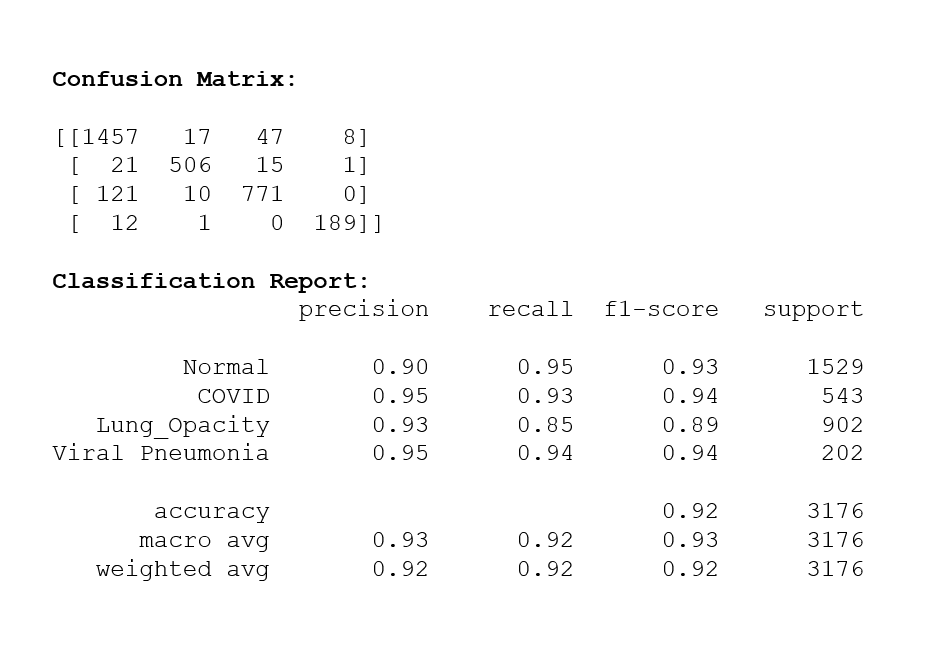
\includegraphics[width=0.5\linewidth]{figures_report_2/cm_cr_ensemble.png}
    \caption{Evaluation for ensemble}
    \label{fig: Confusion matrix for ensemble}
\end{figure}\\


\underline{Grad-CAM and Localization Evaluation}

Grad-CAM visualizations were used to evaluate model interpretability. Observations include:

\begin{table}[H]
\centering
\begin{tabular}{|l|l|p{8cm}|}
\hline
\textbf{Model} & \textbf{Localization Quality} & \textbf{Observations} \\
\hline
VGG16 + Mask & Moderate  & Sometimes focused on non-lung regions such as spine, diaphragm, or borders. \\
\hline
CNN + Stacked Mask & High  & Diffuse, weak heatmaps with limited discriminative ability. \\
\hline
\textbf{Voting Ensemble} & \textbf{High} & Focused and consistent attention on lung regions; better clinical reliability. \\
\hline
\end{tabular}
\caption{Grad-CAM-based qualitative analysis of model attention.}
\end{table}



Figure \ref{fig:Visualization of Gradcam} compares the interpretability and performance of various deep learning models used for chest X-ray classification. The visualizations show heatmaps (via Grad-CAM) that highlight where each model "looks" when making predictions.

\begin{itemize}
    \item A standard VGG16 model achieved 91\% accuracy but displayed diffuse attention patterns, occasionally focusing outside the lung region.
    \item A custom CNN using additional segmentation mask input achieved 92\% accuracy and showed improved focus within the lungs.
    \item An enhanced VGG16 model that applied attention to mask regions delivered the highest single-model accuracy of 94\%, with strong alignment to pathology.
     \item Finally, a voting ensemble model that combines predictions from all three approaches achieved a balanced accuracy of 92\%, leveraging their complementary strengths.
\end{itemize}

Therefore the ensemble model offers more reliable and interpretable insights into model decision-making.

\begin{figure}%[h!] % the [h!] helps force it "here"
    \centering
    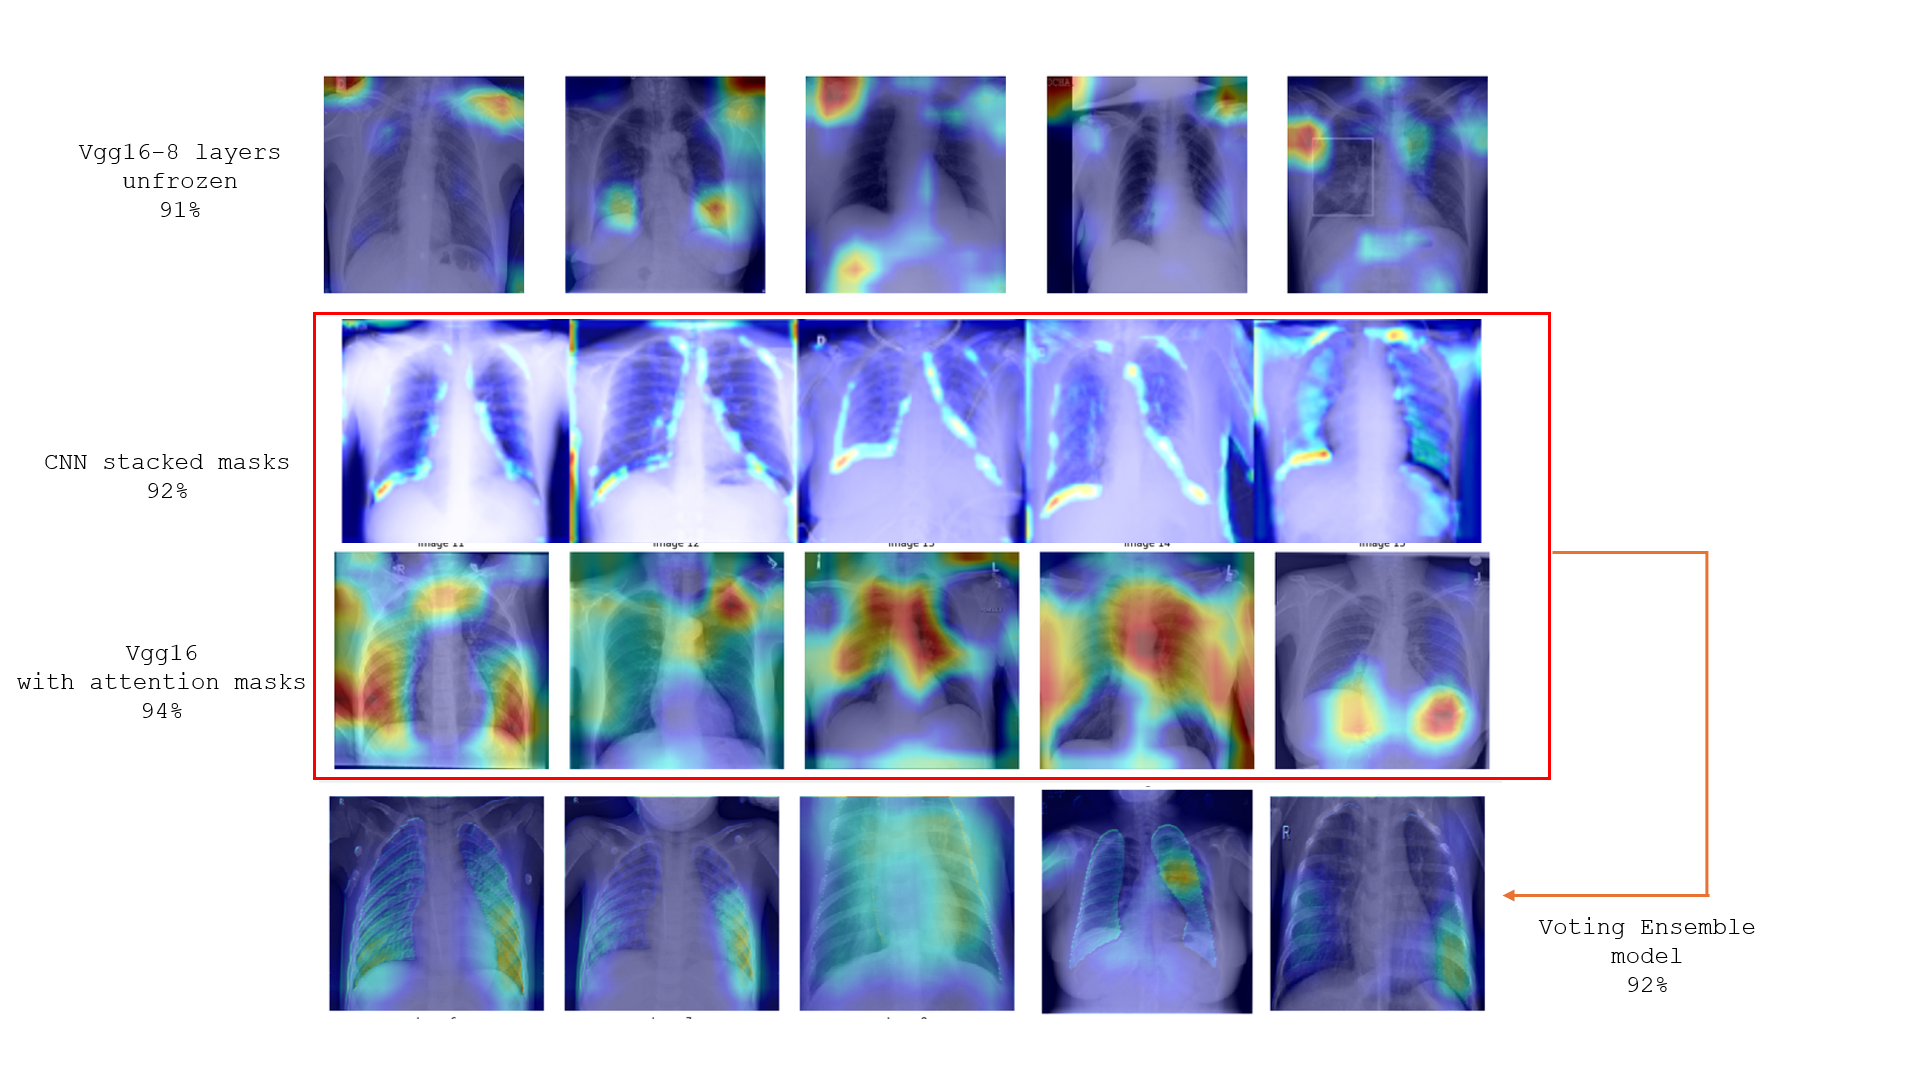
\includegraphics[width=1.0\linewidth]{gradcam_final.png}
    \caption{Visualization Gradcam Improvement}
    \label{fig:Visualization of Gradcam}
\end{figure}




%------------------------------------------------------------------------
% Chapter 4: Conclusion and Future Work
%------------------------------------------------------------------------
\section{Conclusions from the modelling}


%------------------------------------------------------------------------
% Chapter 4.1: Machine Learning vs. Deep Learning for classification of chest X-ray images
%------------------------------------------------------------------------

\subsection{Machine Learning vs. Deep Learning for classification of chest X-ray images}

From the various runs with different machine learning models we came to the conclusion, that it is not possible to use fullsize images (299 x 299 pixels) with these models. 
When trying to use the fullsize images, we had severe performance issues as the trainig comsumed too much RAM which even led to a crash of the model run. Therefore, the image size had to be reduced to e.g. 128 x 128 pixels and for some models even more drastically to even 20 x 20 pixels. A disadvantage of the intensivly reduced pixel number leads to a loss of information in the X-ray images, which could influence the model performance. 

Additionally, for some machine learning models, the number of images used for training also had to be reduced due to performance issues. This reduced the variety of images involved in the training of the model. 

Our tests have shown that machine learning models perform better when using extracted features as input rather than the images themselves. An exception too this is the XGBoost model. A XGBoost model on 128 x 128 images without masks, no filter (Clahe, Gaussian Blur) gave us the best overall accuracy and not the model run using the already extracted features by HOG-technique. 

Despite these limitations, we were even able to achieve relatively good results with machine learning models. (XGBoost with an overall accuracy of 86\% and surprisingly good predictions for the COVID class of 89\%). 
The advantages of these machine learning models were: 
* As they need limited computational resources we could run them on our local computers.
* As training is much faster than using deep learning models, more runs with different parameters and input data could be tested. 

Deep learning offers significant advantages over traditional machine learning for classifying chest X-ray images. These models excel in handling high-dimensional data and they can automatically identify relevant features. Deep learning models, particularly convolutional neural networks (CNNs), learn features directly from raw image data, so that no preprocessing like feature extraction and applying relevant filters has to be done by hand. This ability allows them to capture subtle patterns and complex structures that may be missed by manually designed features. Furthermore, less "man power" is needed for the preprocessing of the images. 

Our tests with several deep learning models showed that we could further improve the accuracy of the predictions to 92\% even for the COVID class we got scores of 93-95\%. When using these models to determine if a patient has COVID or other deseases it is important not to miss out a sick person. Reaching this goal using a model with the highest possible accuracy we assume that the higher computational costs and the more time-consuming training of a deep learning model is acceptable.\\

%------------------------------------------------------------------------
% Chapter 4.2: Which model to
%------------------------------------------------------------------------

\subsection{Which model to chose?}
The best results of each model type are presented in table \ref{tab:model_performance}. The overall accuracy is shown and the scores (precision, recall and f1-score) for the COVID-class. 

\begin{table}[h]
    \centering
    \resizebox{\textwidth}{!}{%
    \begin{tabular}{|l|c|c|c|c|l|}
        \hline
        \textbf{} & \textbf{Overall} & \multicolumn{3}{c|}{\textbf{COVID-class}} & \textbf{Information} \\
        \textbf{} & \textbf{Accuracy} & \textbf{Precision} & \textbf{Recall} & \textbf{F1-score} & \textbf{on Input Data} \\
        \hline
        \multicolumn{6}{|l|}{\textbf{Machine Learning Models}} \\
        \hline
        Logistic Regression & 0.74 & 0.52 & 0.56 & 0.54 & Hog features \\
        Random Forest & 0.76 & 0.62 & 0.61 & 0.62 & Hog features \\
        SVM & 0.57 & 0.45 & 0.43 & 0.44 & Images 128 x 128, 1000 per class \\
        SVM (PCA) & 0.77 & 0.59 & 0.61 & 0.60 & Hog + PCA \\
        XGBoost & 0.86 & 0.89 & 0.89 & 0.89 & 128x128, no masks, no filters \\
        MPL Classifier & 0.83 & 0.69 & 0.69 & 0.69 & ResNet features \\
        \hline
        \multicolumn{6}{|l|}{\textbf{Deep Learning Models}} \\
        \hline
        Self-build CNN & 0.92 & 0.93 & 0.98 & 0.95 &  \\
        EfficientNet & 0.58 & 0.28 & 0.07 & 0.11 &  \\
        InceptionV3 & 0.91 & 0.92 & 0.91 & 0.91 &  \\
        DenseNet121 & 0.85 & 0.73 & 0.90 & 0.81 &  \\
        VGG16 & 0.94 & 0.97 & 0.99 & 0.98 &  \\
        Ensemble & 0.92 & 0.95 & 0.93 & 0.94 &  \\
        \hline
    \end{tabular}
    } % end resizebox
    \caption{Performance of the best models for each model type}
    \label{tab:model_performance}
\end{table}

The first part of the project concentrated on using different machine learning models. Using ML models, we got the best results with a XGBoost model using 128 x 128 images without masks, no filter (Clahe, Gaussian Blur). The overall accuracy was 86\%. This model's classification performance for the COVID-class reached impressive 89\% for precision, recall and f1-score. 

By using deep learning models we could further improve the accuracy of the predictions. The scores of runs with an InceptionV3 model looked very good. This model's best run achieved an overall accuracy of 91\% and even the COVID-class is well predicted (precision 92\%, recall 91\% and f1-score 91\%). However, further inspections of these model revealed that it as convergence problems. 

We also achieved very good results with the VGG16 model. In addition to a high overall accuracy of 91\% and also good results for the COVID class: precision 99\%, recall 82\% and f1-score 90\%, the model showed sufficient convergence. Therefore, this seemed to be the best model and could go for it. Unfortunately a Grad-CAM analysis showed that our most promising model does not only focus on the lung areas of the X-ray images. 

By using attention masks, this VGG16 model improved its focus on lung areas in X-ray images, enhancing classification accuracy. It achieved 94\% overall accuracy, with strong performance in COVID (F1-score: 0.98), Viral Pneumonia (0.98), Normal (0.95), and Lung Opacity (0.91). The macro-averaged F1-score of 0.95 confirmed balanced effectiveness across various pathologies.


\begin{table}[hb]
\centering
\begin{tabular}{|l|c|c|c|}
\hline
\textbf{Model} & \textbf{Accuracy} & \textbf{F1-Score} & \textbf{Localization} \\
\hline
VGG16 + Mask Attention & High & High & Moderate \\
\hline
CNN + Stacked Inputs & Lower & Lower & High \\
\hline
Voting Ensemble & Slightly Lower & Slightly Lower & Best \\
\hline
\end{tabular}
\caption{Performance and localization comparison of different models.}
\label{tab:ensemble_performance}
\end{table}

The voting ensemble model\ref{tab:ensemble_performance}, though slightly lower in raw metrics, demonstrated:

\begin{itemize}
  \item Best localization performance via Grad-CAM
  \item Superior attention to lung regions with reduced artifact reliance
  \item Enhanced clinical trustworthiness and deployment safety
\end{itemize}

\noindent
\textbf{Therefore, the voting ensemble is the recommended model for practical deployment, balancing accuracy, interpretability, and robustness.}






%------------------------------------------------------------------------
% Chapter 5: Discussion - Reflecting on our project
%------------------------------------------------------------------------
\section{Discussion - Reflecting on our project}

\underline{ Overall Model Performance }
\begin{itemize}
    \item Accuracy: 0.9203 → Very high, showing robust performance.
    \item Precision \& Recall: High across all classes, especially COVID and Viral Pneumonia.Slight recall drop for Lung\_Opacity (0.85), indicating some missed true positives.
    \item Confusion Matrix observations:Normal misclassified as Lung\_Opacity: 47 times.Lung\_Opacity misclassified as Normal: 121 times. Suggests confusion between Normal and Lung Opacity, likely due to subtle visual overlaps.
\end{itemize}


\underline{Confidence Analysis (Subfigure a, top-left)}
Per-class Average Confidence:
\begin{itemize}
    \item Viral Pneumonia: 0.7938
    \item COVID: 0.7786
    \item Lung\_Opacity: 0.7041
    \item Normal: 0.5830
\end{itemize}

Interpretation:

The ensemble is less confident when predicting "Normal" — possibly due to overlap with subtle opacity patterns.
Highest confidence in COVID and Viral Pneumonia → good class separation and learning.
Moderate confidence for Lung\_Opacity — matches the lower recall from the confusion matrix.

\begin{figure}%[h!] % the [h!] helps force it "here"
    \centering
    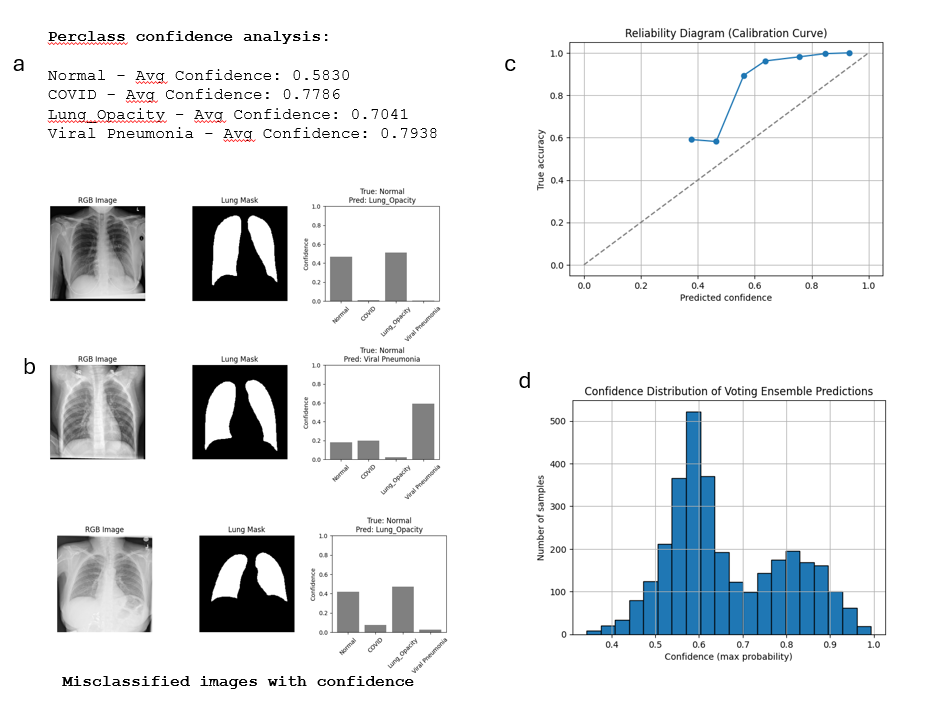
\includegraphics[width=1.0\linewidth]{error_analysis.png}
    \caption{Visualization of model error analysis}
    \label{fig:error_analysis}
\end{figure}

\underline{Misclassified Examples (Subfigures a \& b)}\\

These panels show:
Original X-ray + Lung Mask + Predicted Probabilities
Example b1 and b2:
True: Normal, but predicted:As Lung\_Opacity (b1 and b3) and As Viral Pneumonia(b2)

Insights:
\begin{itemize}
    \item The model assigns considerable confidence to incorrect classes — e.g., >0.6 for Lung\_Opacity in b1.
    \item This supports the earlier finding that Normal - Lung\_Opacity confusion is a key error source.
    \item Lung masks appear similar — suggesting visual ambiguity.
\end{itemize}

\underline{Confidence Histogram (Subfigure d)}

Most predictions fall around 0.55–0.65 range.
Skewed toward moderate confidence, not overly confident.
Indicates model is generally cautious, but some misclassifications occur even with >0.6 confidence.

\underline{Reliability Diagram (Subfigure c)}
Shows how well predicted probabilities align with actual accuracy.
For predicted confidences >0.6, the model is well-calibrated (close to diagonal).
At \~0.5 confidence, accuracy drops, showing lower trustworthiness for moderate scores.


\subsection{Summary \& Recommendations}
\begin{table}[ht]
\centering
\renewcommand{\arraystretch}{1.4}
\begin{tabular}{|p{4.5cm}|p{4.5cm}|p{5.5cm}|}
\hline
\textbf{Insight} & \textbf{Evidence} & \textbf{Action} \\
\hline
Normal $\leftrightarrow$ Lung\_Opacity confusion & Confusion matrix and misclassified images & Enhance training data with clearer Normal \& Opacity samples; use Grad-CAM to verify regions \\
\hline
Low confidence in ``Normal'' class & Per-class average confidence: 0.583 & Revisit data quality or apply augmentations for Normal class \\
\hline
Slight overconfidence at low prediction scores & Reliability curve dips below diagonal & Use \textbf{temperature scaling} or \textbf{Platt scaling} for better confidence calibration \\
\hline
Misclassifications are not always low-confidence & Examples shown in Figure~\ref{fig:error_analysis} (part b) & Consider ensemble thresholding or abstaining from low-confidence predictions \\
\hline
\end{tabular}
\caption{Error analysis insights and proposed actions for improving the voting ensemble model}
\label{tab:error_actions}
\end{table}


In conclusion the model is overconfident at lower probability bins, a common issue.These findings suggest that while the ensemble is highly effective overall, further refinement—particularly in distinguishing between Normal and Lung Opacity cases and improving calibration at lower confidence thresholds—could further enhance its reliability and trustworthiness in clinical decision-making.\\

\section{Difficulties Encountered}

Throughout the course of this project, several technical, computational, and methodological challenges were encountered, which influenced the development timeline and outcomes.

\underline{Scientific Obstacles}
A major scientific challenge was effectively integrating mask information with RGB image data in a way that preserved semantic alignment. Balancing the use of handcrafted features with learned deep representations also required careful experimentation, particularly when designing the ensemble structure to combine the CNN and attention-based VGG16 models.

\underline{Delays and Model Training}
Training the attention-based model introduced unexpected delays. Due to its higher complexity and additional input stream (masks), convergence required significantly more epochs and tuning compared to the baseline CNN. This impacted the project schedule and necessitated changes to the training pipeline.

\underline{Dataset Issues}
We faced notable dataset-related challenges. These included class imbalance (especially fewer samples for the “Viral Pneumonia” class), inconsistent image quality, and the need to preprocess and resize medical images and masks to a consistent resolution. Merging masks and images into model-ready formats also introduced overhead.

\underline{Relevance and Model Selection}
Initial approaches using traditional machine learning (e.g., SVM with HOG features) proved insufficient in capturing the complexity of the imaging data. This led to a shift in focus toward deep learning-based solutions, which better aligned with the project goals but increased computational and implementation demands.

\underline{Computational Constraints}
Working within Google Colab imposed memory and runtime constraints. Model checkpoints, high-resolution image processing, and ensemble predictions all placed significant strain on available GPU and RAM resources. At times, these limitations affected training batch sizes and model saving strategies.

\underline{Other Considerations}
Occasional interruptions in access to cloud resources, syncing issues with Google Drive, and the complexity of managing multiple model files and configurations also added to the logistical load. Moreover, integrating intermediate results from separate models into a unified evaluation pipeline required careful coordination and documentation.



%------------------------------------------------------------------------
% Chapter 6: References
%------------------------------------------------------------------------
\section{References}

-M.E.H. Chowdhury, T. Rahman, A. Khandakar, R. Mazhar, M.A. Kadir, Z.B. Mahbub, K.R. Islam, M.S. Khan, A. Iqbal, N. Al-Emadi, M.B.I. Reaz, M. T. Islam, “Can AI help in screening Viral and COVID-19 pneumonia?” IEEE Access, Vol. 8, 2020, pp. 132665 - 132676.\\
-Rahman, T., Khandakar, A., Qiblawey, Y., Tahir, A., Kiranyaz, S., Kashem, S.B.A., Islam, M.T., Maadeed, S.A., Zughaier, S.M., Khan, M.S. and Chowdhury, M.E., 2020. Exploring the Effect of Image Enhancement Techniques on COVID-19 Detection using Chest X-ray Images. arXiv preprint arXiv:2012.02238. 

%------------------------------------------------------------------------
% Chapter 7: Appendices
%------------------------------------------------------------------------
\section{Appendices}

You can find the GitHub repository belonging to this project here: 
\url{https://github.com/DataScientest-Studio/mar25-bds_analysis-of-covid-19-chest-x-rays}\\
\url{https://bimcv.cipf.es/bimcv-projects/bimcv-covid19/#1590858128006-9e640421-6711}\\
]\url{https://github.com/ml-workgroup/covid-19-image-repository/tree/master/png}\\
\url{https://sirm.org/category/senza-categoria/covid-19/}\\
\url{https://eurorad.org}\\
\url{https://github.com/ieee8023/covid-chestxray-dataset}\\
\url{https://figshare.com/articles/COVID-19_Chest_X-Ray_Image_Repository/12580328}\\
\url{https://github.com/armiro/COVID-CXNet}\\  
\url{https://www.kaggle.com/c/rsna-pneumonia-detection-challenge/data}\\
\url{https://www.kaggle.com/paultimothymooney/chest-xray-pneumonia}\\




\end{document}
